\chapter[\texorpdfstring{\MakeUppercase{Công trình khoa học đã công bố}}{Công trình khoa học đã công bố}]{Công trình khoa học đã công bố}
Phần này liệt kê bài báo khoa học liên quan đến đề tài luận văn (viết chung với ThS. Nguyễn Vũ Thái, TS. Đỗ Trí Nhựt và TS. Nguyễn Văn Dũ), bài báo đã được chấp nhận đăng:

\begin{enumerate}
  \item Thai Nguyen Vu, \textbf{Bui Van Dung}, Tri Nhut Do, Van Du Nguyen, ``A Comparison of Dimensionality Reduction and Feature Selection for Network Intrusion Detection on Apache Spark ML with a Leakage-Aware Evaluation Pipeline,'' National Conference on Fundamental and Applied Information Technology Research (FAIR), 2026.
\end{enumerate}

Hình~\ref{fig:fair_accept} là thư thông báo chấp nhận đăng bài của Ban tổ chức Hội nghị FAIR 2026.

\begin{figure}[htbp]
    \centering
    \IfFileExists{img/fair_2026_accept.png}{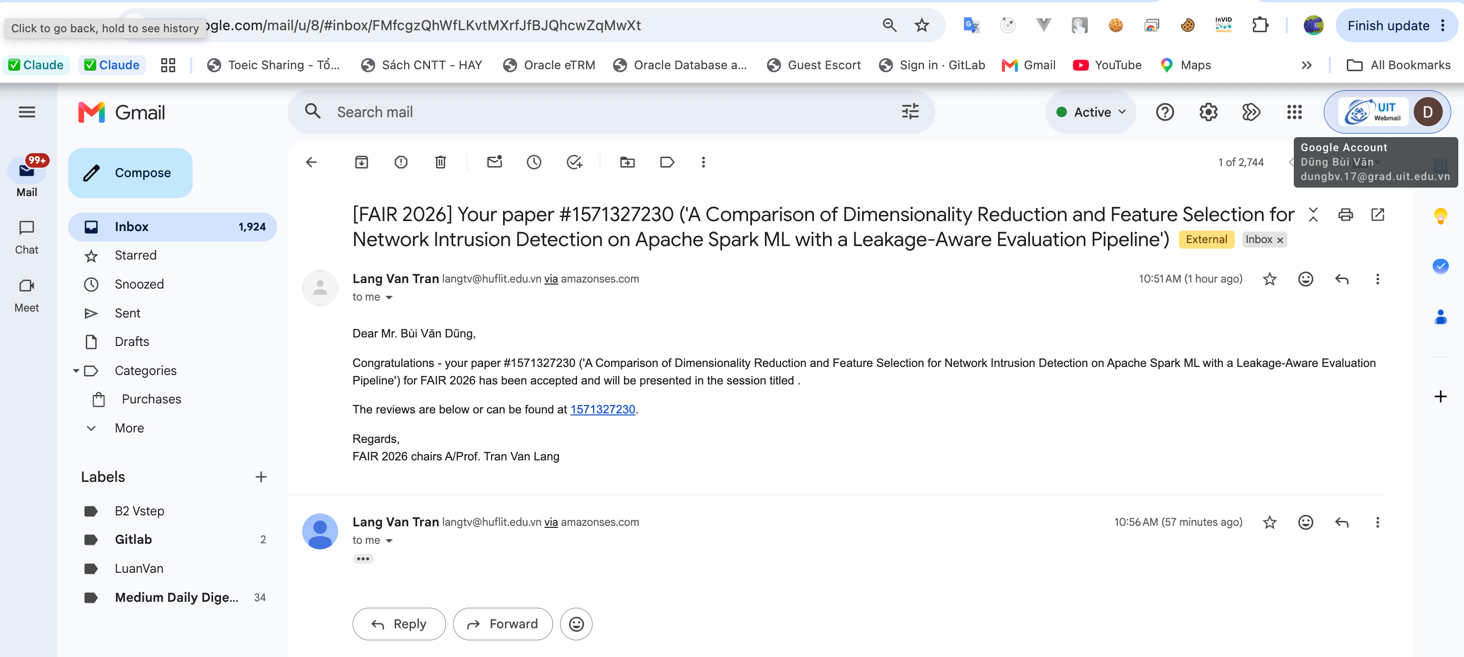
\includegraphics[width=\textwidth]{img/fair_2026_accept.png}}{\fbox{\parbox{0.85\textwidth}{\centering\vspace{1.2cm}\ph{Thư chấp nhận đăng bài của Hội nghị FAIR 2026}\vspace{1.2cm}}}}
    \caption[Thư chấp nhận đăng bài của Hội nghị FAIR 2026]{Thư thông báo chấp nhận đăng bài (paper \#1571327230) của Ban tổ chức Hội nghị FAIR 2026}
    \label{fig:fair_accept}
\end{figure}

Bản PDF đầy đủ của bài báo được đính kèm ở cuối luận văn, sau phần Tài liệu tham khảo. Biên nhận chuyển giao bản quyền bài báo cho IEEE (IEEE Copyright and Consent Form) được đính kèm ngay sau đây.

\IfFileExists{CopyrightReceipt.pdf}{%
  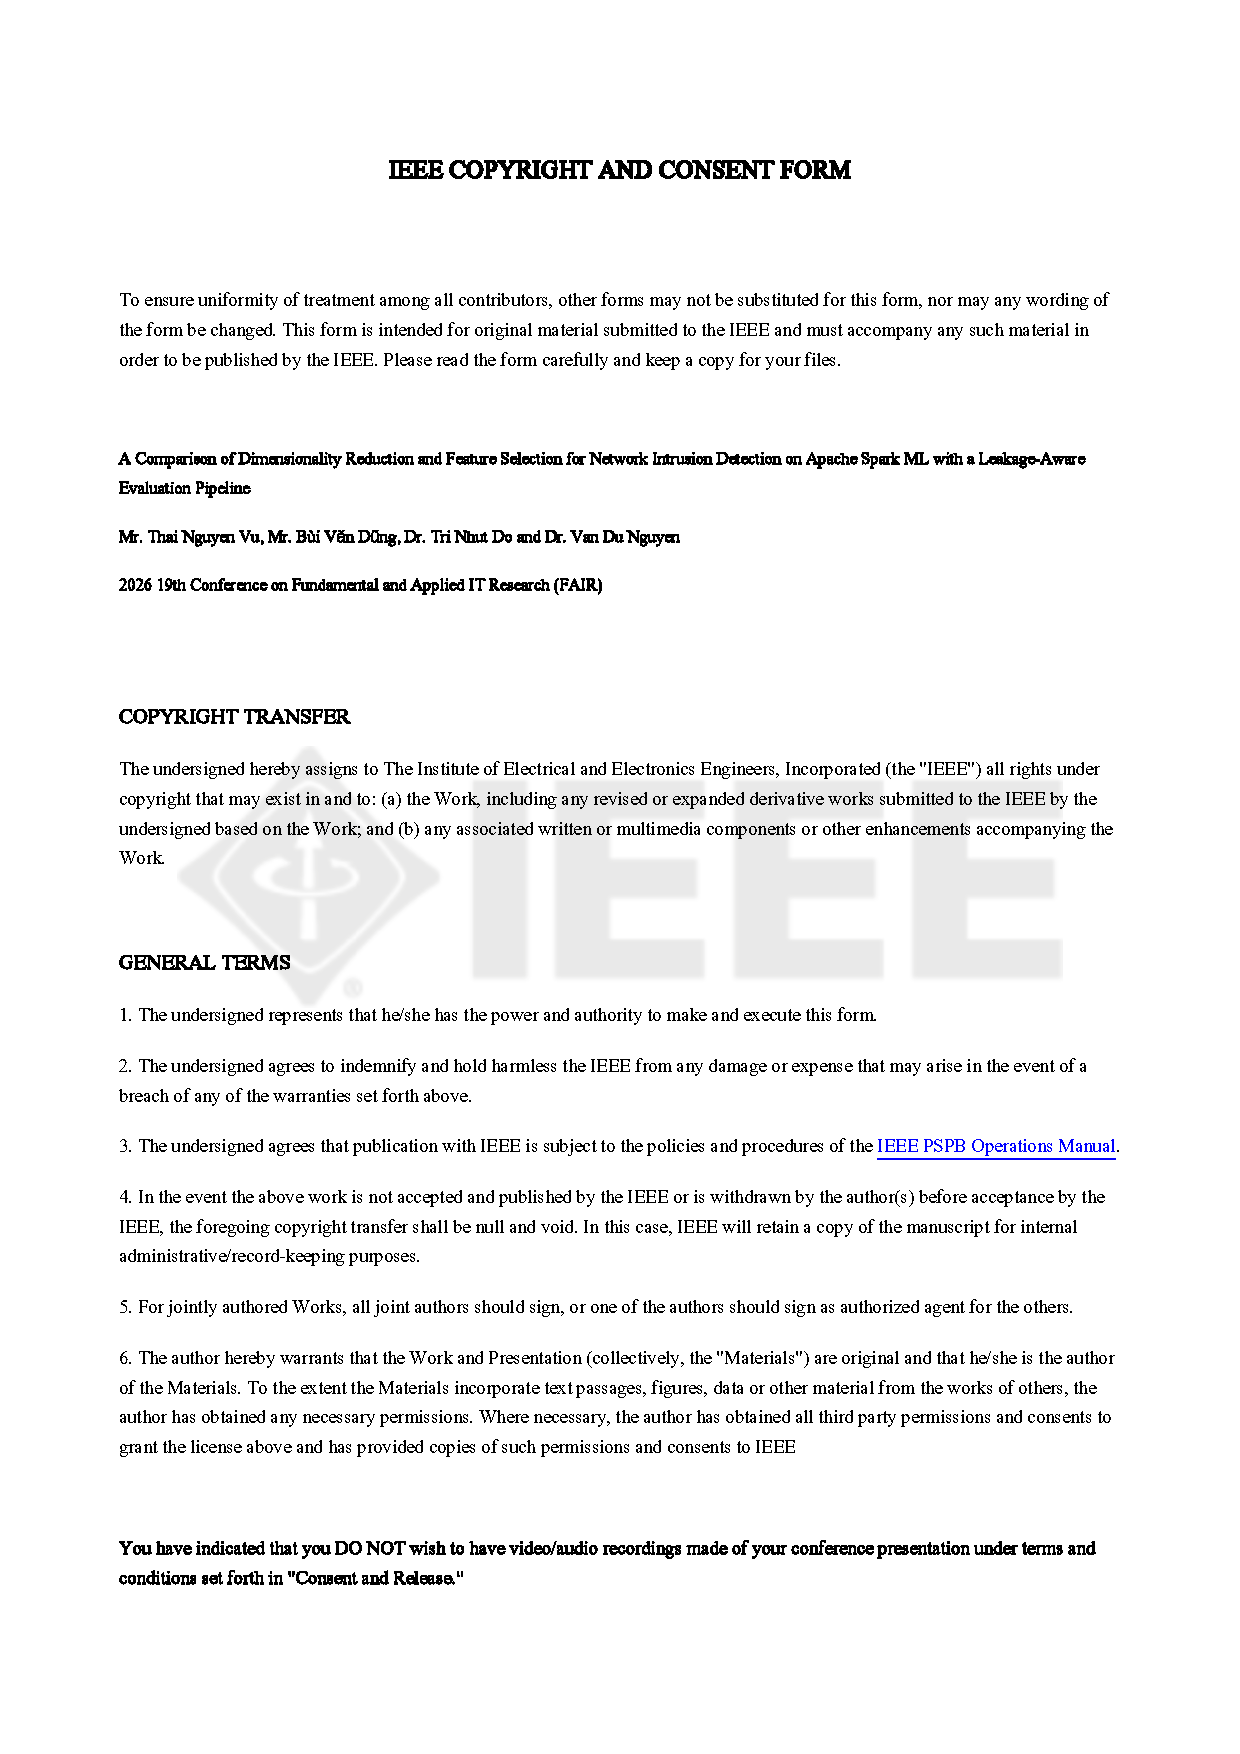
\includepdf[pages=-,scale=0.9,fitpaper=false,pagecommand={\thispagestyle{empty}}]{CopyrightReceipt.pdf}%
}{}